
\documentclass{article}

\usepackage[dvipsnames]{xcolor}
\usepackage{microtype}
\usepackage{graphicx}
\usepackage{caption}
\usepackage{pgfplots}
\usepackage{hyperref}
\usepgfplotslibrary{groupplots}
\captionsetup{singlelinecheck=false}
\definecolor{pastelBlue}{RGB}{0, 114, 178}    %
\definecolor{pastelYellow}{RGB}{230, 159, 0}  %
\definecolor{pastelRed}{RGB}{204, 51, 51} %
\definecolor{pastelGreen}{RGB}{204, 121, 167} %
\usepackage{subcaption}
\usepackage{booktabs} %

%%%%% NEW MATH DEFINITIONS %%%%%

% \usepackage{amsmath,amsfonts,bm}
\usepackage{amsmath,amsfonts}

\usepackage{pifont}


\newcommand{\R}{\mathbb{R}}


\def\va{{\mathbf{a}}}
\def\vg{{\mathbf{g}}}

% Sets
\def\sR{\mathbb{R}}
\def\sC{\mathbb{C}}
\def\sZ{\mathbb{Z}}
\def\sN{\mathbb{N}}
\def\sQ{\mathbb{Q}}

\def\sS{\mathcal{S}}



% Vectors
\def\vzero{{\mathbf{0}}}
\def\vone{{\mathbf{1}}}
\def\vmu{{\mathbf{\mu}}}
\def\vtheta{{\mathbf{\theta}}}
\def\va{{\mathbf{a}}}
\def\vb{{\mathbf{b}}}
\def\vc{{\mathbf{c}}}
\def\vd{{\mathbf{d}}}
\def\ve{{\mathbf{e}}}
\def\vf{{\mathbf{f}}}
\def\vg{{\mathbf{g}}}
\def\vh{{\mathbf{h}}}
\def\vi{{\mathbf{i}}}
\def\vj{{\mathbf{j}}}
\def\vk{{\mathbf{k}}}
\def\vl{{\mathbf{l}}}
\def\vm{{\mathbf{m}}}
\def\vn{{\mathbf{n}}}
\def\vo{{\mathbf{o}}}
\def\vp{{\mathbf{p}}}
\def\vq{{\mathbf{q}}}
\def\vr{{\mathbf{r}}}
\def\vs{{\mathbf{s}}}
\def\vt{{\mathbf{t}}}
\def\vu{{\mathbf{u}}}
\def\vv{{\mathbf{v}}}
\def\vw{{\mathbf{w}}}
\def\vx{{\mathbf{x}}}
\def\vy{{\mathbf{y}}}
\def\vz{{\mathbf{z}}}
\def\vzeta{{\mathbf{\zeta}}}

% Matrix
\def\mA{{\mathbf{A}}}
\def\mB{{\mathbf{B}}}
\def\mC{{\mathbf{C}}}
\def\mD{{\mathbf{D}}}
\def\mE{{\mathbf{E}}}
\def\mF{{\mathbf{F}}}
\def\mG{{\mathbf{G}}}
\def\mH{{\mathbf{H}}}
\def\mI{{\mathbf{I}}}
\def\mJ{{\mathbf{J}}}
\def\mK{{\mathbf{K}}}
\def\mL{{\mathbf{L}}}
\def\mM{{\mathbf{M}}}
\def\mN{{\mathbf{N}}}
\def\mO{{\mathbf{O}}}
\def\mP{{\mathbf{P}}}
\def\mQ{{\mathbf{Q}}}
\def\mR{{\mathbf{R}}}
\def\mS{{\mathbf{S}}}
\def\mT{{\mathbf{T}}}
\def\mU{{\mathbf{U}}}
\def\mV{{\mathbf{V}}}
\def\mW{{\mathbf{W}}}
\def\mX{{\mathbf{X}}}
\def\mY{{\mathbf{Y}}}
\def\mZ{{\mathbf{Z}}}
\def\mBeta{{\mathbf{\beta}}}
\def\mPhi{{\mathbf{\Phi}}}
\def\mLambda{{\mathbf{\Lambda}}}
\def\mSigma{{\mathbf{\Sigma}}}


% Expectation
% \def\eE{\mathop{\mathbb{E}}\limits}
\def\eE{\mathbb{E}}

% Probability
\def\pP{\mathbb{P}}

% Tilde
\def\tf{\tilde{f}}
\def\tS{\tilde{S}}
\def\wtF{\widetilde{\mathcal{F}}}
\def\whR{\widehat{R}}
\def\tvx{\tilde{\mathbf{x}}}
\def\ty{\tilde{y}}


\def\defeq{\overset{\textup{def}}{=}}
% \def\defeq{\overset{.}{=}}
\def\defone{\overset{\text{\ding{172}}}{=}}
\def\deftwo{\overset{\text{\ding{173}}}{=}}
\def\leqone{\overset{\text{\ding{172}}}{\leq}}
\def\leqtwo{\overset{\text{\ding{173}}}{\leq}}
\def\leqthree{\overset{\text{\ding{174}}}{\leq}}
\def\leqfour{\overset{\text{\ding{175}}}{\leq}}
\def\eqone{\overset{\text{\ding{172}}}{=}}
\def\eqtwo{\overset{\text{\ding{173}}}{=}}
\def\eqthree{\overset{\text{\ding{174}}}{=}}
\def\eqfour{\overset{\text{\ding{175}}}{=}}
\def\geqfive{\overset{\text{\ding{176}}}{\geq}}

\usepackage{hyperref}


\newcommand{\theHalgorithm}{\arabic{algorithm}}
\newcommand{\sumtoken}{\textnormal{\texttt{[SEP]}}}
\newcommand{\stag}{s_{\texttt{tag}}}
\newcommand{\snum}{s_{\texttt{num}}}
\DeclareMathOperator{\attention}{Attention}
\DeclareMathOperator{\MHA}{MHA}
\newcommand{\m}[1]{\bm{#1}}           %
\makeatletter
\renewcommand*\env@matrix[1][*\c@MaxMatrixCols c]{%
  \hskip -\arraycolsep
  \let\@ifnextchar\new@ifnextchar
  \array{#1}}
\makeatother


\usepackage[accepted]{icml2025}

\usepackage{amsmath}
\usepackage{amssymb}
\usepackage{mathtools}
\usepackage{amsthm}
\usepackage{mdframed}
\usepackage{changepage}
\usepackage{caption}
\usepackage{enumitem}

\usepackage{tikz}
\usetikzlibrary{chains, arrows.meta, positioning}

\usepackage{bold-extra}
\newcommand{\question}[1]{\textsc{#1}}


\usepackage[capitalize,noabbrev]{cleveref}

\theoremstyle{plain}
\newtheorem{theorem}{Theorem}[section]
\newtheorem{proposition}[theorem]{Proposition}
\newtheorem{lemma}[theorem]{Lemma}
\newtheorem{corollary}[theorem]{Corollary}
\theoremstyle{definition}
\newtheorem{definition}[theorem]{Definition}
\newtheorem{assumption}[theorem]{Assumption}
\theoremstyle{remark}
\newtheorem{remark}[theorem]{Remark}

\usepackage[textsize=tiny]{todonotes}


\icmltitlerunning{A `Catch, Tag, and Release' Mechanism for Embeddings }

\begin{document}


\twocolumn[
\icmltitle{\raisebox{-0.3ex}{\includegraphics[height=0.98em]{fish.png}} Attention Sinks and Outlier Features:\\ A `Catch, Tag, and Release' Mechanism for Embeddings}





\icmlsetsymbol{equal}{*}
\vspace{-0.5em}
\begin{icmlauthorlist}
    \icmlauthor{Stephen Zhang$^{1,2,*}$}{}
    \icmlauthor{Mustafa Khan$^{1,2,*}$}{}
    \icmlauthor{Vardan Papyan$^{1,2}$}{}


\end{icmlauthorlist}

\icmlaffiliation{1}{University of Toronto}

\icmlcorrespondingauthor{Stephen Zhang}{stephenn.zhang@mail.utoronto.ca}

\icmlkeywords{Attention Sink, Outlier Features, LLMs, Pruning, Low-Rank, ICML}

\vskip 0.2in
]




\footnotetext[1]{University of Toronto and $^2$Vector Institute. $^*$Equal contribution. Correspondence to: Stephen Zhang $<$stephenn.zhang@mail.utoronto.ca$>$ and Mustafa Khan $<$mr.khan@mail.utoronto.ca$>$.}

\begin{abstract}
Two prominent features of large language models (LLMs) is the presence of large-norm (outlier) features and the tendency for tokens to attend very strongly to a select few tokens. Despite often having no semantic relevance, these select tokens, called attention sinks, along with the large outlier features, have proven important for model performance, compression, and streaming. Consequently, investigating the roles of these phenomena within models and exploring how they might manifest in the model parameters has become an area of active interest. Through an empirical investigation, we demonstrate that attention sinks utilize outlier features to: \textit{catch} a sequence of tokens, \textit{tag} the captured tokens by applying a common perturbation, and then \textit{release} the tokens back into the residual stream, where the tagged tokens are eventually retrieved. We prove that simple tasks, like averaging, necessitate the `catch, tag, release' mechanism hence explaining why it would arise organically in modern LLMs. Our experiments also show that the creation of attention sinks can be completely captured in the model parameters using low-rank matrices, which has important implications for model compression and substantiates the success of recent approaches that incorporate a low-rank term to offset performance degradation. 
Link to \href{https://catch-tag-release.github.io}{\textcolor{Cerulean}{project page}}.
\end{abstract}


\section{Introduction}
\subsection{`Catch, Tag, and Release' in Aquatic Conservation}
In marine biology, the `catch, tag, and release' mechanism is a vital tool for tracking fish populations. A fish is caught, fitted with a tracking tag encoding critical information, and then released back into a water stream, where it is monitored over time. This enables researchers to understand migration patterns, survival rates, and ecosystem interactions. 



\subsection{Pervasive Phenomena in LLMs}
Remarkably, modern large language models (LLMs) exhibit a strikingly similar mechanism when processing tokens. To understand why, we first examine two recent discoveries in LLM research:\medskip
\begin{mdframed}[shadow=true, shadowsize=1pt]
\textbf{Attention Sinks}: Coined by \citet{xiao2024efficient}, the authors found that all tokens attend strongly to the first token. Follow-up works demonstrated that sinks may also appear in later tokens \citep{yu2024unveiling, sun2024massive, cancedda2024spectralfiltersdarksignals}.
\end{mdframed}

\begin{mdframed}[shadow=true, shadowsize=1pt]
\textbf{Outlier Features}: Feature dimensions in the activations that are significantly larger in magnitude \citep{kovaleva-etal-2021-bert, dettmers2022gptint}. Unlike attention sinks, outlier feature dimensions are consistent across tokens.
\end{mdframed}


\begin{figure*}[t]
    \centering
    \begin{subfigure}{1\textwidth}
        \centering
        \includegraphics[width=0.45\textwidth]{figures/catch.pdf}
        \caption{
        \textbf{Catch:} Attention sinks catch the attention of a subset of tokens, through outlier features, as shown in Figures \ref{fig:sinks} and \ref{fig:outliers}.
        }
        \label{fig:diag_catch}
    \end{subfigure}\vspace{0.2cm}
    \vfill
    \begin{subfigure}{1\textwidth}
        \centering
        \includegraphics[width=0.8\textwidth]{figures/tag.pdf}
        \caption{
        \textbf{Tag:} The attention layer then tags the captured tokens by introducing an outlier feature dimension across all tokens. This shared tag causes tokens to cluster based on the attended sink, e.g. in PCA plots, as shown in Figure \ref{fig:pca_attention_output}.
        }
        \label{fig:diag_tag}
    \end{subfigure}\vspace{0.4cm} 
    \vfill
    \begin{subfigure}{\textwidth}
        \centering
        \includegraphics[width=\textwidth]{figures/release.pdf}
        \caption{
        \textbf{Release:} The tagged tokens are then released into the residual stream, where deeper layers can exploit the tag for further processing. This common tag induces token clustering even in deeper layers, e.g. in PCA plots, as shown in Figure \ref{fig:pca_residual_stream}.
        } 
        \label{fig:diag_release}
    \end{subfigure}\vspace{-0.2cm}
    \caption{An illustration of the `catch, tag, release' mechanism.}
    \label{fig:ctr_diagram}
\end{figure*}



Both phenomena have been linked to model performance, particularly in streaming \citep{xiao2024efficient, guo-etal-2024-attention}, quantization techniques \citep{dettmers2022gptint, son2024prefixingattentionsinksmitigate, ashkboos2024quarot}, and pruning techniques \citep{sun2024a, anonymous2025oats}, as behaviors that need to be preserved in the model's attention weights and features. This, in turn, has driven prior research to investigate the following question.



\subsection{Why Do Sinks and Outliers Emerge?}
Existing answers generally fall into two main categories:
\begin{description}
    \item[To Create Implicit Attention Biases] Models lack explicit bias parameters in the attention layers, leading attention sinks and large outliers to emerge as compensatory mechanisms that artificially introduce such biases. As a result, these effects can be mitigated by incorporating explicit key or value bias parameters \citep{sun2024massive, gu2024attention}.
    \item[To Turn Off Attention Heads] Attention sinks emerge as a learned, data-dependent mechanism that disables an attention head when it is not needed for the current sequence \citep{bondarenko2023quantizable, guo2024activedormantattentionheadsmechanistically}.
\end{description}





\newpage




\subsection{Open Questions}
Both perspectives still leave the following unanswered questions:

\begin{itemize}
    \item[\question{{\large Q}1:}] \textit{How do attention sinks and outlier features manifest in model parameters?}
\end{itemize}
While sinks and outlier features play a crucial role in model compression, prior research has primarily focused on their presence in model embeddings. Their manifestation within model parameters remains largely unexplored, raising questions about the best strategies for preserving these critical properties during compression.

\begin{itemize}
    \item[\question{{\large Q}2:}] \textit{Why do attention sinks emerge in later tokens?}
\end{itemize}
Neither perspective fully explains why attention sinks appear in later tokens alongside the first token sink \citep{yu2024unveiling, cancedda2024spectralfiltersdarksignals}. These sinks are sequence-dependent, contradicting the bias perspective, and the presence of multiple sinks seems unnecessary from the active-dormant perspective.

\begin{itemize}
    \item[\question{{\large Q}3:}] \textit{Are attention sinks beneficial or better dispersed?}
\end{itemize}
It remains unclear whether attention sinks are critical for model performance and need to be preserved \citep{xiao2024efficient, son2024prefixingattentionsinksmitigate}, or if they should be dispersed or removed altogether \citep{sun2024massive, yu2024unveiling}. 














\begin{figure*}[h]
    \centering

    \begin{minipage}{\textwidth}
        \centering
        \begin{subfigure}{0.34\textwidth}
            \includegraphics[width=\textwidth]{figures/Fig_1_Phi3_Medium_PCA_Layer_3_Head_6_Activation_Sink.pdf}
        \end{subfigure}
        \hfill
        \begin{subfigure}{0.61\textwidth}
            \includegraphics[width=\textwidth, trim=0 0 250 0, clip]{figures/Fig_1_Phi3_Medium_PCA_Layer_3_Head_6_Activation_Outlier_CROP.pdf}
            \vspace{-0.1cm}
        \end{subfigure}
    \end{minipage}

    \begin{minipage}{\textwidth}
        \centering
        \begin{subfigure}{0.34\textwidth}
            \caption{\textbf{Attention Weights.} Two distinct attention sinks catch the attention of tokens appearing later in the sequence.}
            \label{fig:sinks}
        \end{subfigure}
        \hfill
        \begin{subfigure}{0.61\textwidth}
            \caption{\textbf{Output of Attention Layer.} The sink token exhibits an outlier feature that is then copied by the attention weights to the caught tokens, creating an outlier feature dimension.}
            \label{fig:outliers}
        \end{subfigure}
    \end{minipage}
    
    \begin{subfigure}[t]{\linewidth}
        \centering
        \vspace{0.4cm}
        \includegraphics[width=\textwidth, trim=5 20 5 20, clip]{figures/Fig_1_Phi3_Medium_PCA_Layer_4_Head_7_Value_Embedding.pdf}
        \caption{
            \textbf{PCA on the output of the attention layer.} Tokens cluster according to their attended sink: those attending to the first sink are shaded red, while those attending to the second sink are shaded green.
        }
        \label{fig:pca_attention_output}
    \end{subfigure}\\
    \begin{subfigure}[b]{\linewidth}
        \centering
        \vspace{0.4cm}
        \includegraphics[width=\textwidth, trim=5 20 5 20, clip]{figures/Fig_1_Phi3_Medium_PCA_Layer_17_Output_Embedding_Final.pdf}
        \caption{
            \textbf{PCA on the residual stream in a deep layer.} Tagged tokens propagate through the residual stream, clustering based on their previously attended sink. Tokens that attended to the first sink are green, while those attending to the second sink are brown and yellow.
        }
        \label{fig:pca_residual_stream}
    \end{subfigure}
    \caption{
        Visualization of the `catch, tag, and release' mechanism. The second and third subplots use PCA-based coloring of embeddings. %
    }
    \label{fig:mainfigure}
\end{figure*}



\newpage


\subsection{Contributions}\label{sec:logic_flow}
Our first contribution is a theoretical study of a two-layer attention model trained to average a sequence of numbers. This analysis answers the questions posed and establishes the following claims, summarized in the schematic below:
\begin{figure}[H]
    \centering
    \begin{center}
    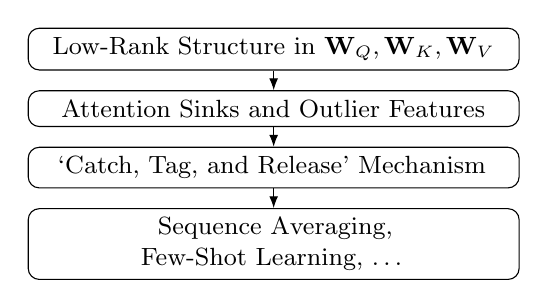
\begin{tikzpicture}[
        node distance=0.25cm,
        every node/.style={draw, text width=6cm, align=center, font=\small, rounded corners},
        every path/.style={draw, -{Latex[length=1.5mm]}}
    ]
    
    \node (lowrank) {Low-Rank Structure in $\mW_Q, \mW_K, \mW_V$};
    \node (sinks) [below=of lowrank] {Attention Sinks and Outlier Features};
    \node (ctr) [below=of sinks] {`Catch, Tag, and Release' Mechanism};
    \node (effects) [below=of ctr] {Sequence Averaging, Few-Shot Learning, \dots};
    
    \path (lowrank) -- (sinks);
    \path (sinks) -- (ctr);
    \path (ctr) -- (effects);
    
    \end{tikzpicture}
    \end{center}
    \label{fig:contributions}
\end{figure}
\begin{itemize}
    \item[\question{{\large A}1:}] A low-rank structure in the attention weight matrices, $\mW_Q, \mW_K, \mW_V$, is responsible for attention sinks and outlier features.
    \item[\question{{\large A}2:}] Attention sinks and outlier features are leveraged by the model to simulate a `catch, tag, and release' mechanism, depicted and explained in Figure \ref{fig:ctr_diagram}.
    \item[\question{{\large A}3:}] The mechanism is useful for averaging a sequence, few-shot learning, and many other tasks.
\end{itemize}
Our second contribution involves showing that pruning algorithms that do not preserve low-rank structure in weight matrices, destroy attention sinks and feature outliers, harm the `catch, tag, release' mechanism, and perform worse on few-shot learning.

\subsection{Relationship with Prior Perspectives}
The `catch, tag, and release' mechanism does not contradict the perspectives on attention sinks presented in prior works by \citet{sun2024massive, gu2024attention, guo2024activedormantattentionheadsmechanistically}. We hypothesize that the prior perspectives are accurately describing the behavior of the attention sink associated specifically with the first token in the sequence. The `catch, tag, and release' mechanism expands on this by describing the behavior associated with the data-dependent sinks that emerge in later tokens \citep{yu2024unveiling}. 





















\section{Evidence for `Catch, Tag, Release'} \label{sec:evidence_catch_tag_release}
This subsection provides empirical evidence for the existence of the `catch, tag, release' mechanism. To this end, we input a prompt
into the Phi-3 Medium model \citep{abdin2024phi-}, and compute various statistics, each offering evidence for the existence of a specific component of the mechanism.

\paragraph{Evidence for Catch} As described in Figure \ref{fig:diag_catch}, the evidence of the catch mechanism amounts to showing the existence of an attention sink. We therefore save the attention weights of layer $3$, head $6$ and plot them in Figure \ref{fig:sinks}. The visualization shows that there are indeed two sinks that are catching the attention of subsequent tokens.  

\paragraph{Evidence for Tag} As described in Figure \ref{fig:diag_tag}, demonstrating the tagging mechanism requires verifying token clustering based on the attended sink. Following \citet{oquab2024dinov}, we compute the top two or three principal components of the $d \times d$ covariance matrix of the attention head outputs, where $d$ is the embedding dimension, and project the embeddings onto this basis. The projected values are then normalized to \([0,255]\) and mapped to RGB channels. Figure \ref{fig:pca_attention_output} illustrates the results, showing a clear grouping of tokens by their attention sinks.


\paragraph{Evidence for Release}
As described in Figure \ref{fig:diag_release}, evidence for release amounts to showing that tokens in the residual stream in deeper layers have the same clustering behavior as exhibited in the attention head output.
We therefore hook the inputs into the feedforward network in layer $17$, and apply the same PCA projection and normalization step as described earlier. The results, presented in Figure \ref{fig:pca_residual_stream}, reveal a similar grouping, providing evidence that the model has utilized the tags generated in the earlier layer. 

Appendix \ref{app:add_exper} presents additional measurements using various prompts including chain-of-thought \citep{wei2022chain}, zero-shot chain-of-thought \citep{fewshot}, among others.



\section{Intervention Through Model Pruning}
This subsection aims to intervene at the root of the logical sequence, displayed in Section \ref{sec:logic_flow}, namely the low-rank structure of the attention weight matrices and to test its effect on the attention sinks and outlier features, the `catch, tag, release' mechanism, and ultimately performance on a down-stream task which relies on it: few-shot learning. The intervention is done through the use of pruning algorithms.

\subsection{How is Pruning Related?}
Pruning algorithms compress models by retaining the fewest possible nonzero parameters while preserving performance \citep{NIPS1988_07e1cd7d, NIPS1989_6c9882bb, NIPS1992_303ed4c6}. However, they typically do not prioritize accurately capturing low-rank structures in the weights.

An exception to this is a recently proposed compression algorithm for LLMs, called OATS \citep{anonymous2025oats}, which approximates the model's weight matrices through a sparse-plus-low-rank decomposition:
\[
\mW \approx \underbrace{\mS}_{\text{Sparse}} + \underbrace{\mU\mV}_{\text{Low-Rank}}\!\!\!\!\mathrlap{^{\top}}\ \ .
\]
This method, by design, explicitly preserves low-rank structures through the low-rank term, a key feature absent from traditional pruning algorithms.

Comparing pruning algorithms with OATS is therefore a natural intervention since it directly controls for the low-rank structure. Having established the intervention, we now test its effect on the attention sinks and outlier features.

\subsection{Low-Rank Terms $\implies$ Sinks and Outliers}
Figure \ref{fig:OATS} presents the attention weights for layer $2$, attention head $6$, of a Phi-3 Medium model in three configurations: a dense model, a model compressed by $50$\% using OATS, and a model compressed by $50$\% using OATS where the low-rank matrices for $\mW_Q, \mW_K, \mW_V$ for that layer are set to $\m0$. The plots reveal clear sinks and outliers, except in the model lacking low-rank terms, suggesting that the low-rank term in OATS is indeed responsible for both phenomena.




    
\subsection{No Low-Rank Terms $\implies$ No Sinks and Outliers}
Figure \ref{fig:pruning} compares the attention weights in layer $36$, head $16$, of a dense Phi-3 Medium model with models that are pruned by $50$\% using OATS, and pruned by $50$\% using Wanda \citep{sun2024a}, and SparseGPT \citep{sparsegpt} -- two methods that do not prioritize a low-rank structure in their formulation. The visualizations reveal that pruning methods like Wanda and SparseGPT lack certain attention sinks found in both the dense and OATS models.


\subsection{Sinks and Outliers $\implies$ `Catch, Tag, and Release'}
The previous two subsections show that classical pruning algorithms fail to retain the low-rank components of attention weights, which results in the loss of attention sinks and outlier features. In contrast, OATS preserves them. Building on Section \ref{sec:evidence_catch_tag_release}, which establishes the necessity of sinks and outliers for the `catch, tag, release' mechanism, we conclude that pruning algorithms like Wanda and SparseGPT break the `catch, tag, release' mechanism, whereas OATS maintains it.

\subsection{`Catch, Tag, and Release' $\implies$ Few-Shot Learning}
Since the `catch, tag, release' mechanism segments sequences, it is likely crucial for distinguishing between examples in few-shot learning. To test this, we measure the gap in $k$-shot performance on the MMLU dataset \citep{hendrycks2021measuring} using LM Harness \citep{eval-harness}, where $k$ ranges from $0$ to $5$. We compare the performance of OATS with Wanda and SparseGPT in Figure \ref{fig:k_shot}.

\begin{figure}[h]
    \centering
    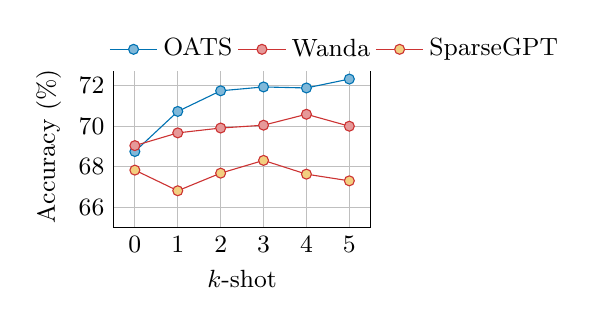
\begin{tikzpicture}
\small
\begin{groupplot}[
    group style={
        group size=1 by 1,
        horizontal sep=0.2cm,
    },
    width=0.4\textwidth,
    height=0.3\textwidth,
    ylabel={Accuracy (\%)},
    xlabel={$k$-shot},
    grid=major,
    domain=0:10,
    legend style={
        legend columns=3,
        font=\small,
        at={(-0.05, 1.1)},
        anchor=west,
        draw=none,
    },
    samples=100,
    ymin=65, ymax=73, %
    xlabel near ticks,
    ylabel near ticks,
]
\nextgroupplot[
    xtick={0, 1, 2, 3, 4, 5},
    xticklabels={0, 1, 2, 3, 4, 5},
    tick style={draw=none},
]
\addplot[mark=*, mark options={fill=pastelBlue!50}, pastelBlue,  mark size=1.8pt]coordinates {
    (0, 68.75)
    (1, 70.73)
    (2, 71.75)
    (3, 71.94)
    (4, 71.89)
    (5, 72.33)
};

\addplot[mark=*, mark options={fill=pastelRed!50}, pastelRed,  mark size=1.8pt] coordinates {
    (0, 69.04)
    (1, 69.67)
    (2, 69.91)
    (3, 70.05)
    (4, 70.59)
    (5, 70.00)
};
\addplot[mark=*, mark options={fill=pastelYellow!50}, pastelRed,  mark size=1.8pt] coordinates {
    (0, 67.83)
    (1, 66.81)
    (2, 67.68)
    (3, 68.31)
    (4, 67.63)
    (5, 67.3)
};
\addlegendentry{OATS}
\addlegendentry{Wanda}
\addlegendentry{SparseGPT}
\end{groupplot}
\end{tikzpicture}
\vspace{-0.25cm}
    \caption{Impact of increasing the number of examples on model performance. Accuracy is measured on the MMLU dataset using 50\% pruned variants of the Phi-3 Medium model.}
    \label{fig:k_shot}
\end{figure}

While all methods perform similarly at $0$-shot, where segmentation is less critical, the gap widens with $k$, highlighting the importance of OATS' ability to retain the `catch, tag, release' mechanism. In contrast, the model pruned by SparseGPT shows no improvement with more examples, indicating severely compromised few-shot capabilities.


\begin{figure*}[t]
    \centering
    \begin{subfigure}[t]{0.3\linewidth}
        \centering
        \includegraphics[width=\linewidth]{figures/oats_components_2/prompt_0_dense_layer_1_head_6_sink.png}
        \includegraphics[width=\linewidth]{figures/oats_components_2/prompt_0_dense_layer_1_head_6_value.png}
            \caption{\centering Dense}
        \label{fig:oats_dense}
    \end{subfigure}
    \hfill
    \begin{subfigure}[t]{0.3\linewidth}
        \centering
        \includegraphics[width=\linewidth]{figures/oats_components_2/prompt_0_oats_layer_1_head_6_sink.png}
        \includegraphics[width=\linewidth]{figures/oats_components_2/prompt_0_oats_layer_1_head_6_value.png}
        \caption{\centering Sparse $+$ Low-Rank}
        \label{fig:oats_full}
    \end{subfigure}
    \hfill
    \begin{subfigure}[t]{0.3\linewidth}
        \centering
        \includegraphics[width=\linewidth]{figures/oats_components_2/prompt_0_sparse_layer_1_head_6_sink.png}
        \includegraphics[width=\linewidth]{figures/oats_components_2/prompt_0_sparse_layer_1_head_6_value.png}
        \caption{\centering Sparse $+ \; \m0$} 
        \label{fig:oats_sparse}
    \end{subfigure}
    \caption{Comparison of attention weights and attention output for layer $2$, head $6$, across the dense Phi-3 Medium, Phi-3 Medium compressed by the OATS algorithm, and Phi-3 Medium compressed by the OATS algorithm with only the sparse terms present in the current layer. The removal of the low-rank term from the $\mW_Q, \mW_K$ fully removes the attention sinks that were present in both the dense model and the model compressed by OATS.} 
    \label{fig:OATS}
\end{figure*}


\begin{figure*}[t]
    \centering
    \begin{subfigure}[b]{0.23\linewidth}
        \centering
        \includegraphics[width=\linewidth]{figures/pruning_sinks/prompt_4_dense_layer_35_head_16.png}
        \caption{\centering Dense Model}
    \end{subfigure}
    \hfill
    \begin{subfigure}[b]{0.23\linewidth}
        \centering
        \includegraphics[width=\linewidth]{figures/pruning_sinks/prompt_4_oats_layer_35_head_16.png}
        \caption{\centering OATS}
    \end{subfigure}
    \hfill
    \begin{subfigure}[b]{0.23\linewidth}
        \centering
        \includegraphics[width=\linewidth]{figures/pruning_sinks/prompt_4_wanda_layer_35_head_16.png}
        \caption{\centering Wanda}
    \end{subfigure}
    \hfill
    \begin{subfigure}[b]{0.23\linewidth}
        \centering
        \includegraphics[width=\linewidth]{figures/pruning_sinks/prompt_4_sparsegpt_layer_35_head_16.png}
        \caption{\centering SparseGPT}
    \end{subfigure}
    \caption{Visualizations of the attention weights of layer 36 head 16 of a Phi-3 Medium that has been compressed by $50$\%. Pruning algorithms that do not prioritize a low-rank structure end up losing an attention sink that is present in both the dense model and OATS.}
    \label{fig:pruning}
\end{figure*}



\section{Theoretical Foundation}
\subsection{Setup and Main Result}
\paragraph{Task} Given a sequence of $T$ tokens, consisting of numbers, $x_i \in \mathbb{R}$, separated by a special \sumtoken token:
$$\vx = (x_1, ..., x_{t-1}, \sumtoken, x_{t+1}, ..., x_T),$$
the objective is to compute the average of the numbers appearing after the \sumtoken token. To increase the complexity of the task, the position of the \sumtoken token, denoted as $t$, varies across different sequences.

\paragraph{Embeddings} The number tokens are embedded into:
$$ \ve_i = \texttt{Embed}(x_i) = \begin{bmatrix} x_i \\ -1 \end{bmatrix} \in \mathbb{R}^2, \quad i\neq t,$$
while the $\sumtoken$ is embedded into:
$$ \ve_t = \texttt{Embed}(\sumtoken) = \begin{bmatrix} s_{\texttt{num}} \\ -s_{\texttt{tag}} \end{bmatrix} \in \mathbb{R}^2,$$
where $s_{\texttt{num}}, s_{\texttt{tag}} \in \mathbb{R}$ are learnable parameters.
The first coordinate of the embeddings represents the numbers, while the second coordinate represents the tag. 

The embeddings are concatenated into a matrix to form:
$$\mE = \begin{bmatrix} \ve_1 & \ve_2 & \cdots & \ve_T \end{bmatrix}^{\top} \in \mathbb{R}^{T\times 2}.$$ 



\paragraph{Model}
The embeddings are passed as input to a two-layer causal transformer:
\begin{align}
    \mH & = \attention(\mE, \mE, \mE\mW^1_V) + \mE \\
    f_{\theta}(\vx) & = \attention(\vh_T^{\top} \mW^2_{Q}, \mH \mW^2_{K}, \mH \mW^2_V),
\end{align}
parameterized by:
$$\theta = (\mW^1_V, \mW^2_{Q}, \mW^2_K, \mW^2_V, s_{\texttt{num}}, s_{\texttt{tag}}).$$
We will use the auxiliary notation:
$$\mA^1 = \softmax(\mE\mE^{\top})$$
$$ \mA^2 = \softmax(\mH\mW^2_Q \mW^2_K\mH^{\top}),$$
where the $\softmax(\cdot)$ is causal. 


\medskip
\begin{mdframed}[shadow=true, shadowsize=1pt, innertopmargin=10pt, innerbottommargin=10pt]
\begin{theorem}[\textbf{`Catch, Tag, and Release' Theory}]
Assume the learnable parameters, $\theta$, satisfy:
\begin{align}
    & \snum =0  \nonumber \\
    & \mW^1_V =\begin{bmatrix} 0 & 0 \\ 0 & -1 \end{bmatrix} \nonumber \\
    & \mW^2_Q\mW^2_K = \begin{bmatrix} 0 & b \\ 0 & d\end{bmatrix}, \ \ \text{where} \ \ d>0, b\in \mathbb{R} \nonumber \\
    & \mW^2_V  = \begin{bmatrix} 1 \\ 0 \end{bmatrix} \label{eqn:wv}
\end{align} 
Then:
$$f_{\theta}(\vx) \stackrel{\stag \to \infty}{\xrightarrow{\hspace{1cm}}} \frac{1}{T-t} \sum_{i=t+1}^{T} x_i$$
for any $x_1,...,x_T \in \mathbb{R}$. The model will have the following features for any sequence $\vx$:
\begin{itemize}
    \item the \!\! \sumtoken \ forms an \textbf{attention sink},
    \item the tokens after the \!\! \sumtoken \ have \textbf{activation outliers} in their second coordinate,
    \item the second coordinate is an \textbf{outlier feature dimension}, and
    \item the attention matrices $\mW^1_V$, $\mW^2_Q$, $\mW^2_K$, $\mW^2_V$ are \textbf{low rank}, projecting either to the tag or number subspace
\end{itemize}
\end{theorem}
\end{mdframed}
\medskip

\begin{remark}
The model utilizes a tagging mechanism based on the second coordinate of the token representations. A token is classified as:
\begin{description}
    \item[\qquad {\textsc{Untagged:}}] if its second coordinate is finite.
    \item[\qquad {\textsc{Tagged:}}] if its second coordinate diverges.
\end{description}
Initially, all number tokens are assumed to be untagged, with their tag coordinate set to \( -1 \).
\end{remark}




\begin{figure}[h]
    \centering
    \includegraphics[width=0.3\textwidth]{figures/attention_sink.pdf}
    \caption{\textbf{Attention probabilities in the first attention layer.} The $\sumtoken$ token acts as an attention sink for tokens $\vx_i$ with $i \geq t$. Consistent with Equation (\ref{eq:exp_decay}), the remaining probabilities in the same rows decay exponentially as $\mathcal{O}(e^{-\stag})$. Notably, the attention sink does not influence the probabilities of tokens $\vx_i$ for $i < t$, which remain $\mathcal{O}(1)$.}
    \label{fig:attention_sink}
\end{figure}



\subsection{Proof of Theorem, Part 1: `Catch, Tag, Release'}
The first part of the proof focuses on the first attention layer.
\paragraph{Catch Mechanism} The attention weight when token $\vx_i$, for $i>t$ is attending to $\sumtoken$ is:
\begin{align*}
    \mA^1_{i,t}
    &= \frac{\exp(\ve_i^{\top} \ve_t)}{\sum_{k=1}^T \exp(\ve_i^{\top}\ve_k)} \\
    &= \frac{\exp(\ve_i^{\top} \ve_t)}{\exp(\ve_i^{\top}\ve_t) + \sum_{k=1, k\neq t}^T \exp(\ve_i^{\top}\ve_k)} \\
    &= \frac{\exp(x_i \snum + \stag)}{\exp(x_i \snum + \stag) + \sum_{k=1, k\neq t}^i \exp(x_ix_k+1)} \\
    &= \frac{\exp(\stag)}{\exp(\stag) + \sum_{k=1, k\neq t}^i \exp(x_ix_k+1)} \stackrel{\stag \to \infty}{\xrightarrow{\hspace{1cm}}} 1.
\end{align*}
Furthermore, for $i>t$ and $j\neq t$:
\begin{align}
\mA^1_{i,j} &= \frac{\exp(1+x_ix_j)}{\exp(\stag) + \sum_{\substack{k=1 \\ k\neq j}}^i \exp(1+x_ix_k)} \in \mathcal{O}(e^{-\stag}) \label{eq:exp_decay}
\end{align}
and therefore:
$$\mA^1_{i,j} \stackrel{\stag \to \infty}{\xrightarrow{\hspace{1cm}}} 0 \quad \text{for} \quad j \neq t.$$
Thus, \sumtoken acts as an attention sink, where all tokens $x_i$ for $i > t$, as well as the $\sumtoken$ token itself, attend exclusively to the \sumtoken token. As a result, the attention of all tokens $x_i$ for $i > t$ and the $\sumtoken$ token have been caught. These observations are depicted in Figure \ref{fig:attention_sink} above.



\paragraph{Tag Mechanism} The attention output of the $i$-th token for $i\geq t$ is:
\begin{align}
    &\attention(\ve_i^{\top}, \mE, \mE\mW^1_V) \nonumber \\
    =&\sum_{j=1}^i \mA^1_{i,j} \ve_j^\top \mW^1_V \nonumber \\
    =&\mA^1_{i, t}\ve_t^\top \mW^1_V + \sum_{j=1, j\neq t}^{i} \mA^1_{i,j} \ve_j^\top \mW^1_V \label{eq:attn} \\
    =&\mA^1_{i, t}\begin{bmatrix}
        0 & \stag
    \end{bmatrix} + \sum_{j=1, j\neq t}^{i} \mA^1_{i,j} \ve_j^\top \mW^1_V
    \stackrel{\stag \to \infty}{\xrightarrow{\hspace{1cm}}} \begin{bmatrix}
        0 & \infty
    \end{bmatrix}. \nonumber
\end{align} 
Recall that the second coordinate of the embeddings represents the tag. The limit above implies that a tag has been created for all tokens $x_i$, for $i>t$. 

After adding the tag to the residual stream, we obtain for $i>t$:
\begin{align}
    \vh_i = \ve_i + \attention(\ve_i^{\top}, \mE, \mE\mW^1_V)^\top \stackrel{\stag \to \infty}{\xrightarrow{\hspace{0.8cm}}} \begin{bmatrix}
        x_i \\ \infty
    \end{bmatrix} \label{eq:residual_stream}
\end{align}
The above implies that all tokens, $x_i$, for $i>t$ have now been tagged. 

\paragraph{Release Mechanism} The tagged tokens have now been released into the residual stream. As we will show in the next subsection, the tags will be leveraged by the second attention layer to generate the desired averaging mechanism.



\subsection{Proof of Theorem, Part 2: Leveraging the Tags}
The second part of the proof focuses on the second attention layer.

The attention weight when token $x_T$ is attending to token $x_j$ is given by:
\begin{align*}
    \mA^2_{T, j} &= \frac{\exp(\vh_T^{\top}\mW^2_Q \mW^2_K\vh_j)}{\sum_{k=1}^T \exp(\vh_T^{\top}\mW^2_Q \mW^2_K\vh_k)}.
\end{align*}
Dividing the numerator and denominator by $\exp(\vh_T^{\top}\mW^2_Q \mW^2_K\vh_T)$, the expression becomes:
\begin{align}
    \mA^2_{T, j} &= \frac{\exp(\vh_T^{\top}\mW^2_Q \mW^2_K\vh_j-\vh_T^{\top}\mW^2_Q \mW^2_K\vh_T)}{\sum_{k=1}^T \exp(\vh_T^{\top}\mW^2_Q \mW^2_K\vh_k-\vh_T^{\top}\mW^2_Q \mW^2_K\vh_T)} \nonumber \\
    &= \frac{\exp(\vh_T^{\top}\mW^2_Q \mW^2_K(\vh_j -\vh_T))}{\sum_{k=1}^T \exp(\vh_T^{\top}\mW^2_Q \mW^2_K(\vh_k - \vh_T))}. \label{eq:attn2}
\end{align}
Consider the term inside the exponent: 
$$\vh_T^{\top}\mW^2_Q \mW^2_K(\vh_j -\vh_T).$$
There are three cases for $j$, depending on whether it is less than, equal to, or greater than $t$. In the next subsection, we prove that
\begin{description}
    \item[\textbf{Case 1:}]
    For $j<t$ (non-tagged tokens),
    $$\exp(\vh_T^{\top}\mW^2_{Q}\mW^2_K(\vh_j - \vh_T)) \stackrel{\stag \to \infty}{\xrightarrow{\hspace{1cm}}} 0.$$
    \item[\textbf{Case 2:}]
    For $j=t$ (sink token),
    $$\exp(\vh_T^{\top}\mW^2_{Q}\mW^2_K(\vh_t - \vh_T)) \stackrel{\stag \to \infty}{\xrightarrow{\hspace{1cm}}} 0.$$
    
    \item[\textbf{Case 3:}]
    For $j > t$ (tagged tokens),
    $$
    \exp(\vh_T^{\top}\mW^2_{Q}\mW^2_K(\vh_j - \vh_T)) \stackrel{\stag \to \infty}{\xrightarrow{\hspace{1cm}}} 1.
    $$
\end{description}
Combining all three cases together with Equation (\ref{eq:attn2}) leads to:
$$\lim_{\stag\to \infty} \mA^2_{T,j} = \begin{cases}
    0, & j < t \\
    0, & j = t\\
    \frac{1}{T-t}, & j > t \\
\end{cases}$$
The above shows how the tags have been leveraged to arrive at a uniform distribution over the desired tokens.
Then using this, Equation (\ref{eq:residual_stream}), and Equation (\ref{eqn:wv}),  we can conclude that:
$$f_{\theta}(\vx) \stackrel{\stag \to \infty}{\xrightarrow{\hspace{1cm}}} \frac{1}{T-t}\sum_{i=1}^{T}x_i.$$



\subsection{Proof of Theorem, Part 3: Proving the Three Cases}

Combining Equation (\ref{eq:attn}) and Equation (\ref{eq:residual_stream}), we get for all $1\leq i \leq T$:
\begin{align*}
    \vh_i^\top &= \ve_i^\top + \mA^1_{i,t} \ve_t^\top \mW^1_V +\sum_{\substack{k=1 \\ k \neq t}}^{i} \mA^1_{i, k}\ve_k^\top \mW^1_V,
\end{align*}
and specifically:
\begin{align*}
& \vh_T^\top = \ve_T^\top + \mA^1_{T,t} \ve_t^\top \mW^1_V +\underbrace{\sum_{\substack{k=1 \\ k \neq t}}^{T} \mA^1_{T, k}\ve_k^\top \mW^1_V}_{\mathcal{O}(e^{-\stag})} \\
\implies & \vh_T = \begin{bmatrix} x_T \\ -1 \end{bmatrix} + \mA^1_{T,t} \begin{bmatrix} 0 \\ \stag \end{bmatrix} + \mathcal{O}(e^{-\stag}).
\end{align*}
Using the two equations above, we get for all $1\leq j \leq T$:
\begin{align*}
\vh_j^\top - \vh_T^\top &= \ve_j^\top -\ve_T^\top + (\mA^1_{j,t} - \mA^1_{T,t})\ve_t^\top \mW^1_V \\
&\quad + \underbrace{\sum_{\substack{k=1 \\ k \neq t}}^{j} \mA^1_{j, k}\ve_k^\top \mW^1_V}_{\mathcal{O}(1) \text{ if } j < t, \text{ otherwise } \mathcal{O}(e^{-\stag})} - \underbrace{\sum_{\substack{k=1 \\ k \neq t}}^{T} \mA^1_{T, k}\ve_k^\top \mW^1_V,}_{\mathcal{O}(e^{-\stag})}
\end{align*}
where the order of magnitude of the last two terms is given by Equation (\ref{eq:exp_decay}) and depicted in Figure \ref{fig:attention_sink}.

Additionally, we will use the fact that for all $j\geq t$:
$$\lim_{\stag \to \infty} d \cdot \mA^1_{T,t}(\mA^1_{j,t} - \mA^1_{T,t})\stag^2 = 0,$$
which we show in Appendix \ref{app:limit_proof}.
\paragraph{Case 1:}
For $j<t$ (non-tagged tokens),
\begin{align*}
    & \vh_T^{\top}\mW^2_{Q}\mW^2_K(\vh_j - \vh_T) \\
    &= \vh_T^{\top}\mW^2_{Q}\mW^2_K\left(\begin{bmatrix} x_j -x_T \\ 0\end{bmatrix} - \mA^1_{T,t} \begin{bmatrix} 0 \\ \stag\end{bmatrix} + \mathcal{O}(1)\right)\\
    &=  \vh_T^{\top}\left(-\mA^1_{T,t}\begin{bmatrix} b\cdot \stag \\ d\cdot \stag\end{bmatrix} +\mathcal{O}(1)\right)\\
    &= \left(\begin{bmatrix} x_T \\ -1\end{bmatrix} + \mA^1_{T,t}\begin{bmatrix}
        0 \\ \stag
    \end{bmatrix} + \mathcal{O}(e^{-\stag})\right)^{\top} \\ 
    &\phantom{=}\quad \left(-\mA^1_{T,t}\begin{bmatrix} b\cdot \stag \\ d\cdot \stag\end{bmatrix} +\mathcal{O}(1)\right) \\
    &=-(\mA^1_{T,t})^2 \cdot d \cdot \stag^2  + \mathcal{O}(\stag) \\
    & \stackrel{\stag \to \infty}{\xrightarrow{\hspace{1cm}}} -\infty, \text{ since } d > 0.
\end{align*}

\paragraph{Case 2:}
For $j=t$ (sink token),
\begin{align*}
    & \vh_T^{\top}\mW^2_{Q}\mW^2_K(\vh_t - \vh_T) \\
    &= \vh_T^{\top}\mW^2_{Q}\mW^2_K\bigg(\begin{bmatrix} 0-x_T \\ -\stag + 1\end{bmatrix} \\
    & \qquad + (\mA^1_{t,t} - \mA^1_{T,t}) \begin{bmatrix} 0 \\ \stag\end{bmatrix} \quad + \mathcal{O}(e^{-\stag})\bigg)\\
    &=  \vh_T^{\top}\bigg(\begin{bmatrix} b\cdot (1-\stag) \\ d\cdot(1-\stag)\end{bmatrix} \\
    & \qquad + (\mA^1_{t,t} - \mA^1_{T,t}) \begin{bmatrix} b\cdot \stag \\ d \cdot \stag\end{bmatrix} + \mathcal{O}(e^{-\stag})\bigg)\\
    &= -\mA^1_{T,t} \cdot d \cdot \stag^2 \\
    & \qquad + \underbrace{d \cdot \mA^1_{T,t}(\mA^1_{t,t} - \mA^1_{T,t})\stag^2}_{\stackrel{\stag \to \infty}{\xrightarrow{\hspace{1cm}}} 0} + \mathcal{O}(\stag) \\
    & \stackrel{\stag \to \infty}{\xrightarrow{\hspace{1cm}}} -\infty.
\end{align*}

\paragraph{Case 3:}
For $j > t$ (tagged tokens),
\begin{align*}
    & \vh_T^{\top}\mW^2_{Q}\mW^2_K(\vh_j - \vh_T) \\
    &= \vh_T^{\top}\mW^2_{Q}\mW^2_K\bigg(\begin{bmatrix} x_j -x_T \\ 0 \end{bmatrix} + \\
    & \qquad + (\mA^1_{j,t} - \mA^1_{T,t}) \begin{bmatrix} 0 \\ \stag\end{bmatrix} + \mathcal{O}(e^{-\stag})\bigg)\\
    &=  \vh_T^{\top}\left((\mA^1_{j,t} - \mA^1_{T,t})\begin{bmatrix} b\cdot \stag \\ d \cdot \stag\end{bmatrix} + \mathcal{O}(e^{-\stag})\right)\\
    &= (\mA^1_{j,t} - \mA^1_{T,t})(x_T \cdot b \cdot \stag - d\cdot \stag) \\
    & \quad + d\cdot \mA^1_{T,t}(\mA^1_{j,t} - \mA^1_{T,t})\stag^2\\
    & \quad +\mathcal{O}(\stag e^{-\stag}) \\
    & \stackrel{\stag \to \infty}{\xrightarrow{\hspace{1cm}}} 0,
\end{align*}
where $\lim_{\stag \to \infty}(\mA^1_{j,t} - \mA^1_{T,T})\stag = 0$ is proved in Appendix \ref{app:limit_proof}.



\section{Related Work}
    \paragraph{Register Buffers in Transformers} \citet{darcet2024vision} observed that vision transformers exhibit high-norm outlier tokens, similar to LLMs, and that registers (data-independent tokens) are needed to prevent them from arising. This aligns closely with the perspective proposed by \citet{sun2024massive, gu2024attention} that the first token attention sink is serving as a bias term for the attention mechanism.  
    \paragraph{Adam Causes Sinks and Outliers} Another recent avenue of investigation is whether attention sinks and outlier feature dimensions are a by-product of the optimizer. Both \citet{kaul2024attentionactivationunravellingenigmas} and \citet{guo2024activedormantattentionheadsmechanistically}, show that the Adam optimizer \citep{adam} leads to attention sinks and outlier features. In the former, they propose OrthoAdam which applies a rotation to the gradients to prevent any specific outlier dimensions. 
    \paragraph{Rank Collapse} Recent studies have shown that stacking self-attention layers in transformers can lead to rank collapse, where token representations lose dimensionality due to inherent architectural properties \citep{noci2022signalpropagationtransformerstheoretical, emergence-of-clusters-rigollet}. This phenomenon may stem from the `catch, tag, release' mechanism, in which attention concentrates around attention sinks, causing tokens to cluster around them and become confined to a low-rank subspace.
    \paragraph{Low-Rank Terms for Model Compression} Beyond OATS, other works have also proposed leveraging low-rank terms to mitigate compression loss for deep networks \citep{reconstruct_slr, mozaffari2024slimoneshotquantizedsparse, li2024svdquant}.  Another line of research is to incorporate a low-rank adapter during compression that is fine-tuned to mitigate drops in performance \citep{pmlr-v202-li23ap, zhang2023pruning, guo2024lqlora, zhao2024apt, mozaffari2025slopedoubleprunedsparseplus}. 



\section{Conclusion}
This paper establishes that low-rank structures in attention weight matrices cause attention sinks and outlier features, which, in turn, enable the `catch, tag, and release' mechanism. This mechanism serves as a fundamental organizational principle in transformers, dynamically segmenting and tagging token sequences to facilitate tasks such as few-shot learning and chain-of-thought reasoning. Empirically, we demonstrate that pruning techniques that fail to preserve low-rank structures disrupt this mechanism, significantly impairing few-shot generalization. Through rigorous theoretical analysis, we prove that `catch, tag, and release' is not incidental but necessary for performing fundamental tasks like averaging a sub-sequence of numbers. This provides a compelling explanation for why this phenomenon emerges organically in transformer architectures.

 



\section*{Acknowledgements}  
This research was supported in part by the Province of Ontario, the Government of Canada through CIFAR, and industry sponsors of the Vector Institute (\url{www.vectorinstitute.ai/partnerships/current-partners/}). This research was also enabled in part by support provided by Compute Ontario (\url{https://www.computeontario.ca}) and the Digital Research Alliance of Canada (\url{https://alliancecan.ca}).








\bibliography{example_paper}
\bibliographystyle{plainnat}


\newpage
\appendix
\onecolumn



\section{Proof of Auxiliary Limits}\label{app:limit_proof}
We first show that:

$$\lim_{\stag \to \infty} d \cdot \mA^1_{T,t}(\mA^1_{t,t} - \mA^1_{T,t})\stag^2 = 0$$
By definition:
$$\mA^1_{T,t} = \frac{\exp(\stag)}{\exp(\stag) + \sum_{k=1, k\neq t}^{T}\exp(x_Tx_k + 1) } =\frac{1}{1 + \sum_{k=1, k\neq t}^{T}\exp(x_Tx_k + 1-\stag) }  $$
and that:
$$ \mA^1_{t,t} = \frac{\exp(\stag^2)}{\exp(\stag^2) + (t-1)\exp(\stag) } =  \frac{1}{1 + (t-1)\exp(\stag-\stag^2) }.$$
Thus, 
$$\mA^1_{t,t} - \mA^1_{T,t} =  \frac{\sum_{k=1, k\neq t}^{T}\exp(x_Tx_k + 1-\stag) - (t-1)\exp(\stag-\stag^2)}{\left(1 + (t-1)\exp(\stag-\stag^2) \right)\cdot \left(1 + \sum_{k=1, k\neq t}^{T}\exp(x_Tx_k + 1-\stag) \right)}$$
Then:
$$\lim_{\stag \to \infty}\stag^2(\mA^1_{t,t} - \mA^1_{T,t}) =  \lim_{\stag \to \infty}\frac{\sum_{k=1, k\neq t}^{T}\stag^2\exp(x_Tx_k + 1-\stag) - (t-1)\stag^2\exp(\stag-\stag^2) }{\left(1 + (t-1)\exp(\stag-\stag^2) \right)\cdot \left(1 + \sum_{k=1, k\neq t}^{T}\exp(x_Tx_k + 1-\stag) \right)} = \frac{0}{1} = 0$$
The rest follows from the fact that $\lim_{\stag\to \infty}\mA^{1}_{T,t} = 1$ and applying basic limit laws. 

We now show similarly that for $j>t$:
$$ \lim_{\stag \to \infty}(\mA^1_{j,t} - \mA^1_{T,T})\stag = 0, \qquad \lim_{\stag \to \infty}(\mA^1_{j,t} - \mA^1_{T,T})\stag^2 = 0$$
Observe that for $j>t$:
$$\mA^1_{j,t} = \frac{\exp(\stag)}{\exp(\stag) + \sum_{k=1, k\neq t}^{j} \exp(x_jx_k +1)} = \frac{1}{1 + \sum_{k=1, k\neq t}^{j} \exp(x_jx_k +1-\stag)} $$
Then
\begin{align*}
    \lim_{\stag \to \infty}(\mA^1_{j,t} - \mA^1_{T,T})\stag &= \frac{\sum_{k=1, k\neq t}^{T}\stag\exp(x_Tx_k + 1-\stag) - \sum_{k=1, k\neq t}^{j} \stag\exp(x_jx_k +1-\stag) }{\left(1 + \sum_{k=1, k\neq t}^{j} \exp(x_jx_k +1-\stag)\right)\cdot \left(1 + \sum_{k=1, k\neq t}^{T}\exp(x_Tx_k + 1-\stag)\right)} \\
    &= \frac{0}{1} = 0
\end{align*}
and similarly,
\begin{align*}
    \lim_{\stag \to \infty}(\mA^1_{j,t} - \mA^1_{T,T})\stag^2 &= \frac{\sum_{k=1, k\neq t}^{T}\stag^2\exp(x_Tx_k + 1-\stag) - \sum_{k=1, k\neq t}^{j} \stag^2\exp(x_jx_k +1-\stag) }{\left(1 + \sum_{k=1, k\neq t}^{j} \exp(x_jx_k +1-\stag)\right)\cdot \left(1 + \sum_{k=1, k\neq t}^{T}\exp(x_Tx_k + 1-\stag)\right)} \\
    &= \frac{0}{1} = 0
\end{align*}



\newpage



\section{Further Experimental Results} \label{app:add_exper}

\vfill
\begin{figure*}[h]
    \centering

    \begin{subfigure}[t]{\linewidth}
        \centering
        \includegraphics[width=0.8\textwidth, trim=5 20 5 20, clip]{figures/supplementary/referential/supplementary_phi3_medium_layer_3_head_30_input_embedding.pdf}
        \caption{\centering Input embedding visualization at layer 3. The visualization does not display any meaningful clustering prior to the tagging mechanism.}
    \end{subfigure}\\\bigskip

    \begin{subfigure}[t]{.48\linewidth}
        \centering
        \includegraphics[width=0.35\textwidth]{figures/supplementary/referential/supplementary_phi3_medium_layer_3_head_30_attention_sink.pdf}
        \caption{\centering Attention probabilities at layer 3, head 30.}
    \end{subfigure}
    \begin{subfigure}[t]{.48\linewidth}
        \centering
        \includegraphics[width=1\textwidth, trim=0 0 180 0, clip]{figures/supplementary/referential/supplementary_phi3_medium_layer_3_head_30_activation_outlier.pdf}
        \caption{\centering Activation outliers in attention output at layer 3, head 30.}
    \end{subfigure}\\\bigskip

    \begin{subfigure}[t]{\linewidth}
        \centering
        \includegraphics[width=0.8\textwidth, trim=5 20 5 20, clip]{figures/supplementary/referential/supplementary_phi3_medium_layer_3_head_30_value_embedding.pdf}
        \caption{\centering Value embedding at layer 3, head 30.}
    \end{subfigure}\\\bigskip
    
    \begin{subfigure}[t]{\linewidth}
        \centering
        \includegraphics[width=0.8\textwidth, trim=5 20 5 20, clip]{figures/supplementary/referential/supplementary_phi3_medium_layer_18_output_embedding.pdf}
        \caption{\centering PCA on residual stream at layer 18.}
    \end{subfigure}

    \caption{Visualization of the `catch, tag, release' mechanism on a sample prompt.}
\end{figure*}

\vfill

\begin{figure*}[h]
    \centering

    \begin{subfigure}[t]{\linewidth}
        \centering
        \includegraphics[width=0.8\textwidth, trim=5 20 5 20, clip]{figures/supplementary/zero-shot-cot/supplementary_phi3_medium_layer_3_head_6_input_embedding.pdf}
        \caption{\centering PCA on the input embeddings to attention layer 3.}
    \end{subfigure}\\\bigskip

    \begin{subfigure}[t]{.35\linewidth}
        \centering
        \includegraphics[width=0.67\textwidth]{figures/supplementary/zero-shot-cot/supplementary_phi3_medium_layer_3_head_6_attention_sink.pdf}
        \caption{\centering Attention weights of layer 3, head 6.}
    \end{subfigure}
    \begin{subfigure}[t]{.64\linewidth}
        \centering
        \includegraphics[width=1\textwidth, trim=0 5 230 0, clip]{figures/supplementary/zero-shot-cot/supplementary_phi3_medium_layer_3_head_6_activation_outlier.pdf}
        \caption{\centering Output of attention layer 3, head 6.}
    \end{subfigure}\\\bigskip

    \begin{subfigure}[t]{\linewidth}
        \centering
        \includegraphics[width=0.8\textwidth, trim=5 20 5 20, clip]{figures/supplementary/zero-shot-cot/supplementary_phi3_medium_layer_3_head_6_value_embedding.pdf}
        \caption{\centering PCA on the output of attention layer 3, head 6.}
    \end{subfigure}\\\bigskip

    \begin{subfigure}[t]{\linewidth}
        \centering
        \includegraphics[width=0.8\textwidth, trim=5 20 5 20, clip]{figures/supplementary/zero-shot-cot/supplementary_phi3_medium_layer_3_head_6_output_embedding.pdf}
        \caption{\centering PCA on the residual stream at layer 3 after the attention layer.}
    \end{subfigure}\\\bigskip
    

    \begin{subfigure}[t]{.48\linewidth}
        \centering
        \includegraphics[width=0.6\textwidth]{figures/supplementary/zero-shot-cot/supplementary_phi3_medium_layer_38_head_33_attention_sink.pdf}
        \caption{\centering Attention sink at layer 38, head 33, \\ highlighting ``Let's think step by step''.}
    \end{subfigure}\\\bigskip
    
    \begin{subfigure}[t]{1\linewidth}
        \centering
        \includegraphics[width=0.8\textwidth, trim=5 20 5 20, clip]{figures/supplementary/zero-shot-cot/supplementary_phi3_medium_layer_38_output_embedding.pdf}
        \caption{\centering PCA on the residual stream at layer 38, preserving earlier tagging effects.}
    \end{subfigure}

    \caption{Visualization of the `catch, tag, release' mechanism in Zero-Shot Chain of Thought (CoT) prompt. Later layers reveal an attention sink forming on ``Let's think step by step'', with the output embedding reflecting earlier tagged value embeddings.}
\end{figure*}

\vfill

\begin{figure*}[h]
    \centering
    
    \begin{subfigure}[t]{\linewidth}
        \centering
        \includegraphics[width=0.8\textwidth, trim=5 20 5 20, clip]{figures/supplementary/cot-example-2/supplementary_phi3_medium_layer_5_head_16_input_embedding.pdf}
        \caption{\centering PCA on the input embeddings to attention layer 5.}
    \end{subfigure}\\\bigskip
    
    \begin{subfigure}[t]{.32\linewidth}
        \centering
        \includegraphics[width=0.67\textwidth]{figures/supplementary/cot-example-2/supplementary_phi3_medium_layer_5_head_16_attention_sink.pdf}
        \caption{\centering Attention weights of layer 5, head 16.}
    \end{subfigure}
    \begin{subfigure}[t]{.67\linewidth}
        \centering
        \includegraphics[width=1\textwidth]{figures/supplementary/cot-example-2/supplementary_phi3_medium_layer_5_head_16_activation_outlier.pdf}
        \caption{\centering Output of attention layer 5, head 16.}
    \end{subfigure}\\\bigskip
    
    \begin{subfigure}[t]{\linewidth}
        \centering
        \includegraphics[width=0.8\textwidth, trim=5 20 5 20, clip]{figures/supplementary/cot-example-2/supplementary_phi3_medium_layer_5_head_16_value_embedding.pdf}
        \caption{\centering PCA on the output of attention layer 5, head 16.}
    \end{subfigure}\\\bigskip
    
    \begin{subfigure}[t]{\linewidth}
        \centering
        \includegraphics[width=0.8\textwidth, trim=5 20 5 20, clip]{figures/supplementary/cot-example-2/supplementary_phi3_medium_layer_21_head_16_output_embedding.pdf}
        \caption{\centering PCA on the residual stream at layer 21.}
    \end{subfigure}

    \caption{Visualization of the `catch, tag, release' mechanism on a Chain of Thought (CoT) prompt.}
\end{figure*}
\vfill


\begin{figure*}[h]
    \centering
    
    \begin{subfigure}[t]{\linewidth}
        \centering
        \includegraphics[width=0.8\textwidth, trim=5 20 5 20, clip]{figures/supplementary/zero-shot-cot-example-2/supplementary_phi3_medium_layer_5_head_14_input_embedding.pdf}
        \caption{\centering PCA on the input embeddings to attention layer 5.}
    \end{subfigure}\\\bigskip
    
    \begin{subfigure}[t]{.28\linewidth}
        \centering
        \includegraphics[width=0.67\textwidth]{figures/supplementary/zero-shot-cot-example-2/supplementary_phi3_medium_layer_5_head_14_attention_sink.pdf}
        \caption{\centering Attention weights at layer 5, head 14.}
    \end{subfigure}
    \begin{subfigure}[t]{.7\linewidth}
        \centering
        \includegraphics[width=1\textwidth, trim=0 0 120 0, clip]{figures/supplementary/zero-shot-cot-example-2/supplementary_phi3_medium_layer_5_head_14_activation_outlier.pdf}
        \caption{\centering Output of attention layer 5, head 14.}
    \end{subfigure}\\\bigskip
    
    \begin{subfigure}[t]{\linewidth}
        \centering
        \includegraphics[width=0.8\textwidth, trim=5 20 5 20, clip]{figures/supplementary/zero-shot-cot-example-2/supplementary_phi3_medium_layer_5_head_14_value_embedding.pdf}
        \caption{\centering PCA on the output of attention layer 5, head 14.}
    \end{subfigure}\\\bigskip
    
    \begin{subfigure}[t]{\linewidth}
        \centering
        \includegraphics[width=0.8\textwidth, trim=5 20 5 20, clip]{figures/supplementary/zero-shot-cot-example-2/supplementary_phi3_medium_layer_18_head_14_output_embedding.pdf}
        \caption{\centering PCA on the residual stream at layer 18.}
    \end{subfigure}\\\bigskip

    \begin{subfigure}[t]{.48\linewidth}
        \centering
        \includegraphics[width=0.6\textwidth]{figures/supplementary/zero-shot-cot-example-2/supplementary_phi3_medium_layer_39_head_24_attention_sink.pdf}
        \caption{\centering Attention sink at layer 39, head 24, \\ highlighting ``Let's think step by step''.}
    \end{subfigure}\\\bigskip
    \begin{subfigure}[t]{1\linewidth}
        \centering
        \includegraphics[width=0.8\textwidth, trim=5 20 5 20, clip]{figures/supplementary/zero-shot-cot-example-2/supplementary_phi3_medium_layer_39_head_24_output_embedding.pdf}
        \caption{\centering PCA on residual stream at layer 39, preserving earlier tagging effects.}
    \end{subfigure}

    \caption{Visualization of the `catch, tag, release' mechanism on a Zero-Shot Chain of Thought (CoT) prompt. Later layers reveal an attention sink forming on "Let's think step by step", with the output embedding retaining features from tagged value embeddings.}
\end{figure*}


\vfill

\begin{figure*}[h]
    \centering
    
    \begin{subfigure}[t]{\linewidth}
        \centering
        \includegraphics[width=0.8\textwidth, trim=5 20 5 20, clip]{figures/supplementary/cot/supplementary_phi3_medium_layer_3_head_30_input_embedding.pdf}
        \caption{\centering PCA on the input embeddings to attention layer 3.}
    \end{subfigure}\\\bigskip
    
    \begin{subfigure}[t]{.38\linewidth}
        \centering
        \includegraphics[width=0.67\textwidth]{figures/supplementary/cot/supplementary_phi3_medium_layer_3_head_30_attention_sink.pdf}
        \caption{\centering Attention weights of layer 3, head 30.}
    \end{subfigure}
    \begin{subfigure}[t]{.6\linewidth}
        \centering
        \includegraphics[width=1\textwidth]{figures/supplementary/cot/supplementary_phi3_medium_layer_3_head_30_activation_outlier.pdf}
        \caption{\centering Output of attention layer 3, head 30.}
    \end{subfigure}\\\bigskip
    
    \begin{subfigure}[t]{\linewidth}
        \centering
        \includegraphics[width=0.8\textwidth, trim=5 20 5 20, clip]{figures/supplementary/cot/supplementary_phi3_medium_layer_3_head_30_value_embedding.pdf}
        \caption{\centering PCA on the output of attention layer 3, head 30.}
    \end{subfigure}\\\bigskip
    
    
    \begin{subfigure}[t]{\linewidth}
        \centering
        \includegraphics[width=0.8\textwidth, trim=5 20 5 20, clip]{figures/supplementary/cot/supplementary_phi3_medium_layer_16_output_embedding.pdf}
        \caption{\centering PCA on the residual stream at layer 16.}
    \end{subfigure}

    \caption{Visualization of the `catch, tag, release' mechanism on a Chain of Thought (CoT) prompt.}
\end{figure*}

\vfill



\clearpage

\section{Experiment Details}
We use the HuggingFace Transformers library to load the models utilized in our experiments \citep{hf_models}. 
\subsection{Pruning Hyperparameters}
For all pruning experiments, we prune uniformly across all linear layers in the model, excluding the embedding and head layers, remaining consistent with \citep{sparsegpt, sun2024a, anonymous2025oats}. As calibration data, we use 128 sequences of length 2048 from the first shard of the C4 dataset \citep{2019t5}. The algorithm-specific hyperparameters are: 
\begin{itemize}
    \item SparseGPT
    \begin{itemize}
    \item Hessian Dampening: $0.1$
    \item Block Size: $128$ 
    \end{itemize}
    \item OATS
    \begin{itemize}
        \item Iterations: $80$
        \item Rank Ratio: $0.25$
    \end{itemize}
\end{itemize}
The prompt used to generate Figure \ref{fig:pruning} is:
\begin{quote}
\texttt{Read the following paragraph and determine if the hypothesis is true. \textbackslash n \textbackslash n Premise: A: Oh, oh yeah, and every time you see one hit on the side of the road you say is that my cat. B: Uh-huh. A: And you go crazy thinking it might be yours. B: Right, well I didn't realize my husband was such a sucker for animals until I brought one home one night. Hypothesis: her husband was such a sucker for animals. Answer: }
\end{quote}
which we sourced from \citet{yu2024unveiling}.


\end{document}
